\documentclass{article}
\usepackage[utf8]{inputenc}
\usepackage[top=3cm, bottom=3cm, left=3cm,right=3cm]{geometry}
%\usepackage[numbers,round]{natbib}
\usepackage{natbib}
\setcitestyle{aysep={}} 
\usepackage{graphicx}
\usepackage{color}
\usepackage{amsmath}
\usepackage{setspace}
\usepackage{amsmath}
\usepackage{mathtools}
\usepackage{bbm}
\usepackage{float}
\usepackage{hyperref}
\usepackage[super]{nth}

\parindent0cm
\parskip0.5cm
\hyphenpenalty=10000
\pretolerance=10000
\usepackage{lineno}
\linenumbers
\linespread{1.5}

\makeatletter
\newcommand{\customlabel}[2]{
\protected@write \@auxout {}{\string \newlabel {#1}{{#2}{}}}}
\makeatother

%\renewcommand\footnote[2][]{\relax}

\begin{document}
{\Large Diagnostics of dated phylogenies in microbial population genetics}


\vspace*{2cm}
Xavier Didelot$^{1,2,*}$, Jake Carson$^{3}$, Paolo Ribeca$^{4,5}$, Erik Volz$^6$

\vspace*{2cm}
$^1$ School of Life Sciences, University of Warwick, United Kingdom\\
$^2$ Department of Statistics, University of Warwick, United Kingdom\\
$^3$ Mathematics Institute, University of Warwick, United Kingdom\\
$^4$ UK Health Security Agency, London, United Kingdom\\
$^5$ Biomathematics and Statistics Scotland, The James Hutton Institute, Edinburgh, United Kingdom\\
$^6$ MRC Centre for Global Infectious Disease Analysis, Department of Infectious Disease Epidemiology, Imperial College London, London, United Kingdom\\
$^*$ Corresponding author. Tel: 0044 (0)2476 572827. Email: \verb+xavier.didelot@warwick.ac.uk+

\newpage
\section*{ABSTRACT}
Microbial population genetic studies often involve the use of a dated phylogeny
to show how the genomes are related over a relevant timescale. 
Many tools have recently been developed to date
the nodes of a standard phylogeny, but all make underlying assumptions that may
not be realistic for a given dataset, making the results potentially unreliable. 
Model comparison is sometimes used to remedy this, whereby inference
under several models is compared to establish which result can be trusted.
Although such comparison is clearly useful to assess the relative merits
of several inference attempts, here instead we focus on the problem
of evaluating how good an inference is in absolute terms, without comparison.
We consider several approaches for diagnosing potential issues
in a reconstructed dated phylogeny, including outlier detection, 
posterior predictive checking and residual analysis. These methods are
well-established diagnostics tools in other areas of statistics, but here
we show how they can be applied to the specific inference of
dated phylogenies. We illustrate their use on many simulated and real datasets.
We advocate the use of these diagnostics tools for all microbial population genetic
studies that involve the reconstruction of a dated phylogeny.

\newpage
\section*{INTRODUCTION}

Dated phylogenies, also known as tip-calibrated, time-stamped or time-calibrated phylogenies, have become a ubiquitous tool in the study of microbial population genetics 
\citep{Drummond2003,Biek2015,rieuxInferencesTipcalibratedPhylogenies2016}. In a dated phylogeny, the branch lengths are measured in a unit of time, for example years or days,
rather than a unit of evolution as in a standard phylogeny. Consequently, the tips of a dated phylogeny are aligned with the (typically known) dates of sampled genomes and
the internal nodes are aligned with the (typically inferred) dates of common ancestors between the genomes.
Many tools exist to build dated phylogenies, either from a sequence alignment using for example BEAST \citep{Suchard2018} or BEAST2 \citep{Bouckaert2019}, or by
dating the nodes of a standard phylogeny, using for example 
LSD \citep{To2016}, node.dating \citep{Jones2017}, treedater \citep{Volz2017}, BactDating \citep{Didelot2018} and TreeTime \citep{Sagulenko2018}.
The dated phylogeny is interesting in itself since it depicts the ancestral relationships of sampled genomes
over time, but it is also often used as the foundation for further analysis \citep{Didelot2022}, such as inference
of demographics \citep{Baele2016}, phylogeography \citep{Lemey2009} 
or transmission between hosts \citep{Didelot2017}.

There are many factors that can invalidate the results of a dated phylogenetics analysis.
One potential issue that has been well studied is whether the temporal signal is 
strong enough for dating to be performed, or in other words whether the population
is measurably evolving \citep{Drummond2003,Biek2015}. Several tests have been proposed
to test the significance of the temporal signal, such as testing the correlation between
sample dates and root-to-tip distances in an undated tree \citep{Rambaut2016a},
comparing results with and without randomizing the sample dates \citep{Duchene2015a} and
comparing results with correct sample dates and with all sample dates forced equal 
\citep{Rambaut2000,Duchene2020}. 
Another possible source of problem concerns the confounding effect that population structure can have on dating 
\citep{Duchene2015a,Murray2016}. This is especially true when the substructures are 
imbalanced \citep{ducheneTreeImbalanceCauses2015}, are sampled
at different dates \citep{tongComparisonMethodsEstimating2018}, have different clock rates
\citep{wertheimInconsistenciesEstimatingAge2012}  and when the population structure is strong 
\citep{navascuesElevatedSubstitutionRate2009}. 
More generally, any dating makes assumptions, often unstated, about the underlying dated tree model 
and the molecular clock model, and if these assumptions are not met the results can be incorrect.

One approach that has been used to ensure that there are no incorrect assumptions being made 
is to perform inference under multiple models and perform model comparison,
typically by computing a Bayes Factor \citep{Baele2012,Li2012,bouckaertBModelTestBayesianPhylogenetic2017}. 
However, this requires multiple runs under different models, and only provides a relative measure
of model appropriateness, with no indication of how good the best model actually is in absolute terms.
In other words, it may be the case that inference under a given model is less incorrect than other attempts,
but still not correct enough to be of any biological value. 

Here we focus on an alternative approach, in which we seek to evaluate
the correctness of an inference and detect if there are any reasons to believe that the inference is not valid.
This approach is sometimes referred to as model checking, model diagnostics or model validation, 
and it is complementary with the model comparison methodology mentioned above. 
We propose several new methods for diagnosing potential problems in dated phylogenies.
We use simulated datasets to test their ability to detect a range of problems
in the inference, including the aforementioned confounding effect of population structure
\citep{Murray2016}. 
We also demonstrate the usefulness of this approach in practice on real datasets.

%\section*{NEW APPROACHES}
%
%The relationship between the different conceptual methods
% used in this paper is illustrated in Figure \ref{fig:flowchart}.  
% Bayesian inference of a dated phylogeny from an undated phylogeny,
% as performed for example using BactDating \citep{Didelot2018}, is shown in Figure \ref{fig:flowchart}A,
% whereas maximization inference, as performed for example using
% LSD \citep{To2016} or treedater \citep{Volz2017}, is shown in Figure \ref{fig:flowchart}B.
% 
% \begin{figure}[p!]
%\begin{center}
%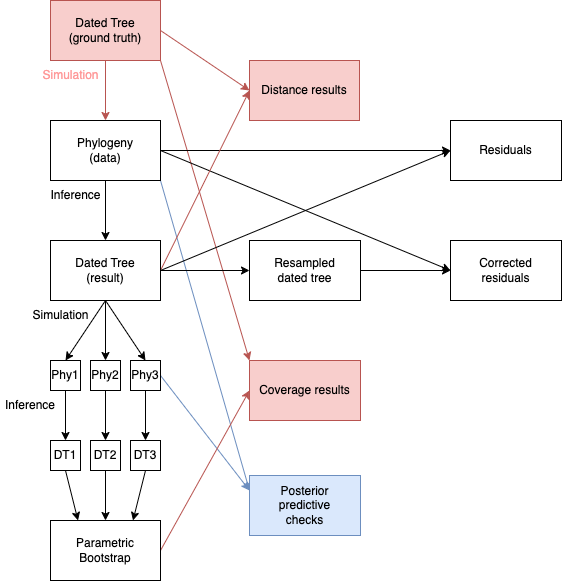
\includegraphics[width=15cm]{flowchart.png}
%\end{center}
%\caption{Concepts used in diagnostics of dated phylogenies. (A) Flowchart for Bayesian methods.
%(B) Flowchart for maximizing methods. Methods using the ground truth are shown in red.
%Posterior predictive checks are shown in blue. Methods based on residuals are shown in green.
%\label{fig:flowchart}}
%\end{figure}
% 
% The ground truth is not known in real applications, but is typically known when simulating
% data for the purpose of testing inference methods. In that case, 
% it is possible to compute the distance between this ground truth and
% the inferred dated phylogeny, with smaller values indicating better performance. 
% However, the absolute (rather than relative) 
% interpretation of this distance can be difficult, which means it is only really
% useful when comparing different inferences from the same dataset. 
%A related concept often used when performing Bayesian inference is coverage.
%For example, when inferring a single parameter value, the coverage represents
%how often the true value is contained within a credible interval. This concept can be used
%when the ground truth is known to validate the dating of a phylogeny inferred using
%Bayesian methods (Figure \ref{fig:flowchart}A) and can also be extended to maximizing methods
%of a parametric bootstrap \citep{efronBayesianInferenceParametric2012} is used to quantify the uncertainty 
%(Figure \ref{fig:flowchart}B).
%

\section*{RESULTS}

\subsection*{Outlier detection analysis}

\begin{figure}[p!]
\begin{center}
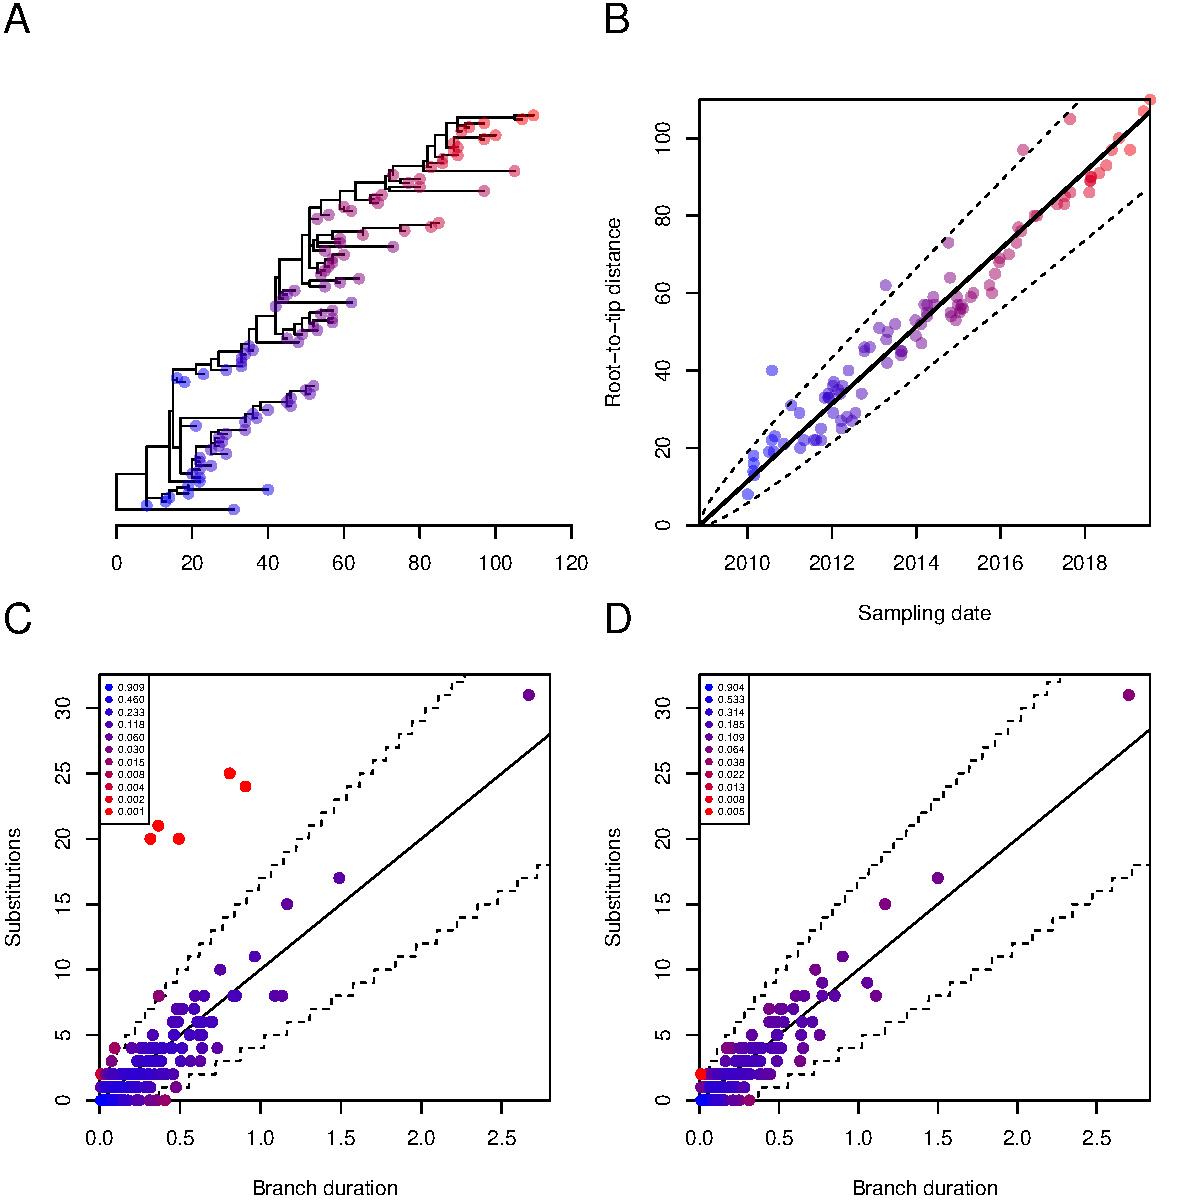
\includegraphics[width=10cm]{outlier.pdf}
\end{center}
\caption{Example of diagnosis using outlier detection.
(A) Simulated phylogeny with 5 outliers. 
(B) Root-to-tip regression analysis.
(C) Distribution of substitutions per branch before removing outliers.
(D) Distribution of substitutions per branch after removing outliers.
\label{fig:outlier}}
\end{figure}

Before dating a phylogeny, it is useful to test the temporal signal by computing a linear regression
between the known isolation dates of the tips and the distances from each tip to the root 
(assuming for now that the root is known). A frequently used software for this analysis is TempEst,
which also allows the detection of outliers as potential problems \citep{Rambaut2016a}. 
For example, in an analysis of 260 genomes from the current pandemic of \textit{Vibrio cholerae},
17 genomes were found to be outliers in the root-to-tip analysis which was 
explained by the fact they were hypermutators \citep{Didelot2015}. A similar outlier detection
approach was implemented in treedater with the difference that it is 
applied to the distribution of likelihood per branch and compared to its expected distribution \citep{Volz2017}.

To illustrate the use of these outlier detection methods,  
a dated phylogeny was simulated including 100 leaves uniformly distributed between 2010 and 2020, 
under the heterochronous coalescent model \citep{Drummond2002}
with constant population size $N_\mathrm{e}g=1$ year. 
We applied a strict clock model (Equation \ref{eq:sc}) to this dated phylogeny,
with clock rate $\mu=10$ substitutions per year, except that for five randomly selected leaves
we added 20 substitutions, resulting in the phylogeny shown in Figure \ref{fig:outlier}A.
The analysis of root-to-tip distances is shown in Figure \ref{fig:outlier}B, with all five modified tips
clearly visible but close to the upper bound of the 95\% expected envelope. 
When treedater was applied to this dataset, all five outliers were detected and given multiple testing corrected
p-values between $8.1\cdot10^{-8}$ and $3.9\cdot10^{-3}$. Figure \ref{fig:outlier}C shows for each
branch of the treedater reconstructed tree its duration, number of substitutions and likelihood.
The five outliers are clearly visible. When the five outliers were removed and treedater rerun,
the resulting Figure \ref{fig:outlier}D looked much more satisfactory.

\subsection*{Posterior predictive analysis}

\begin{figure}[p!]
\begin{center}
A\hspace*{10cm}~\\
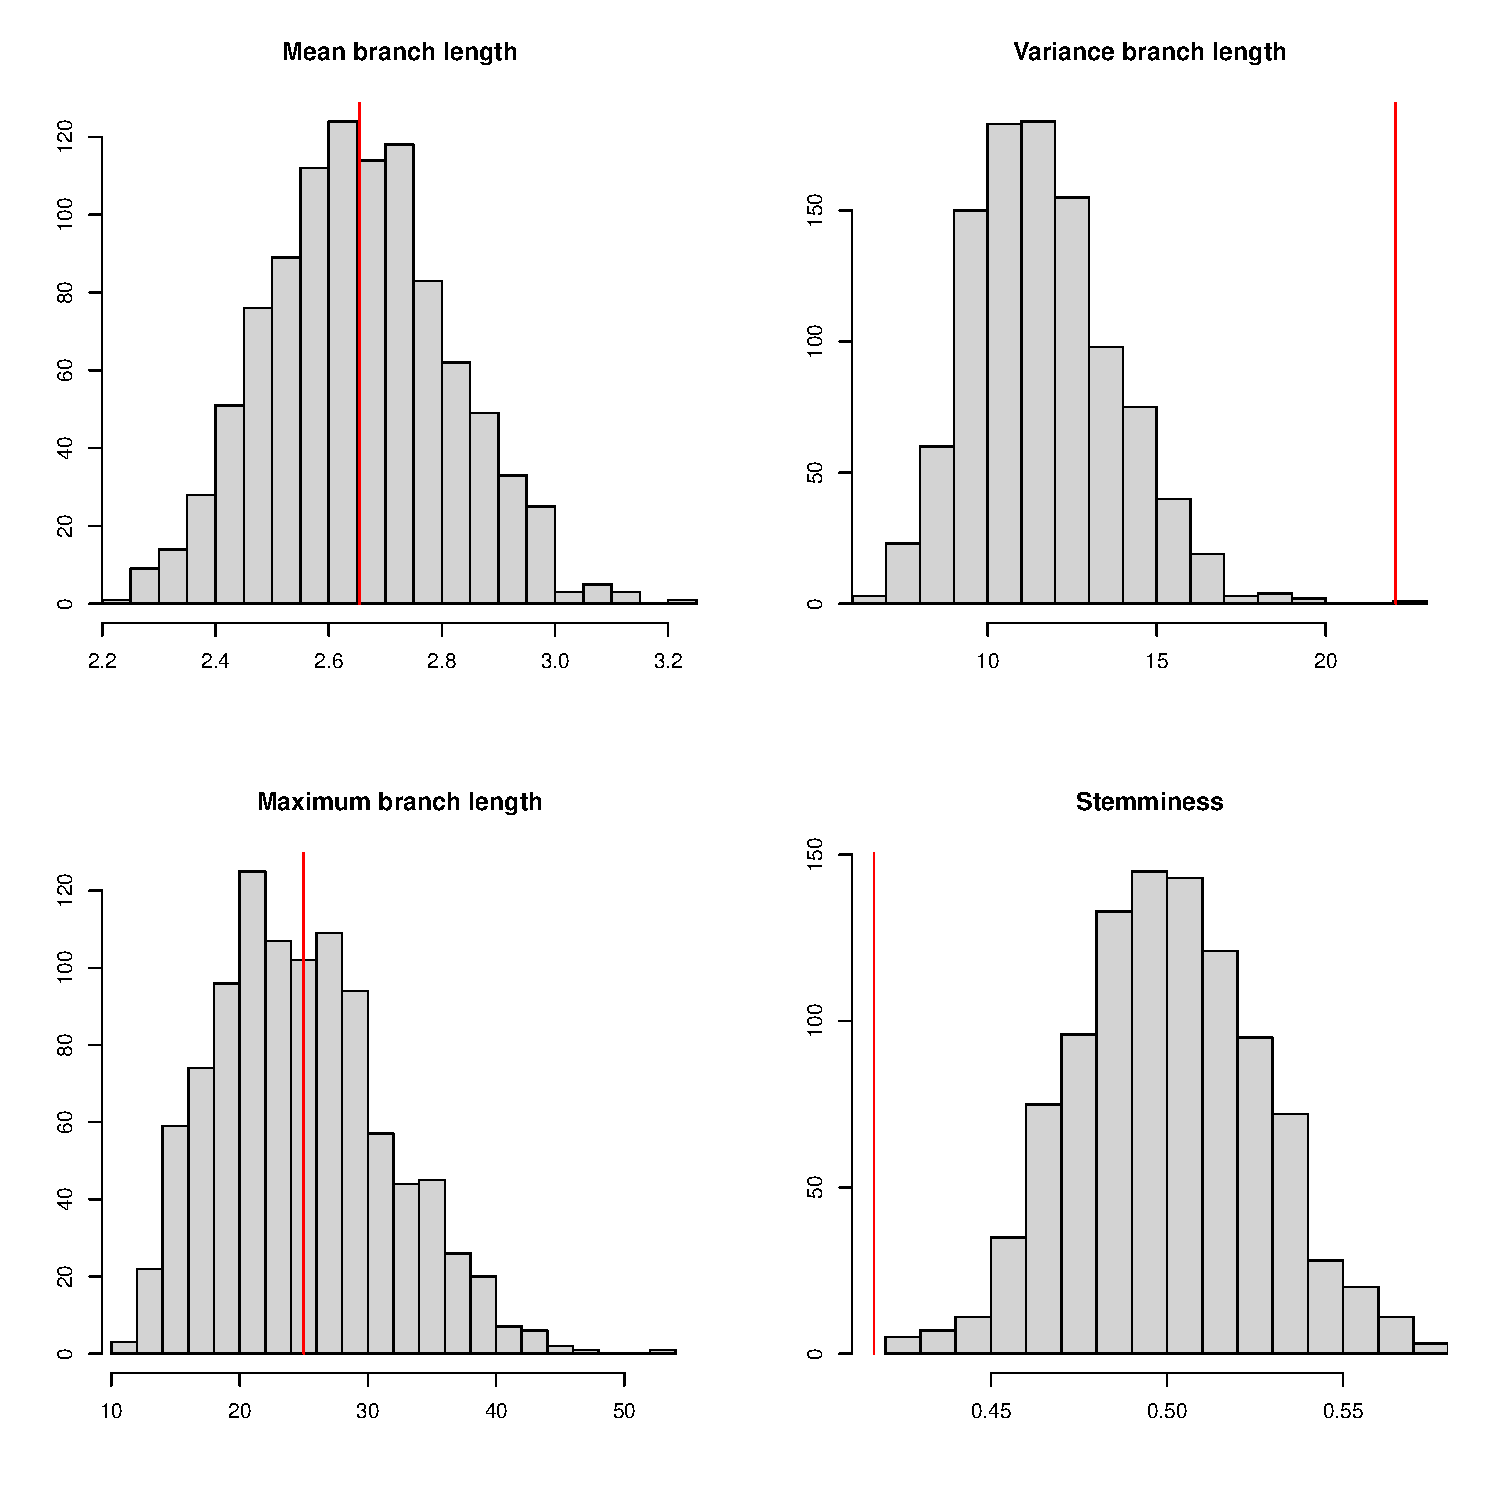
\includegraphics[width=10cm]{examplePPCheck1.pdf}
\\B\hspace*{10cm}~\\
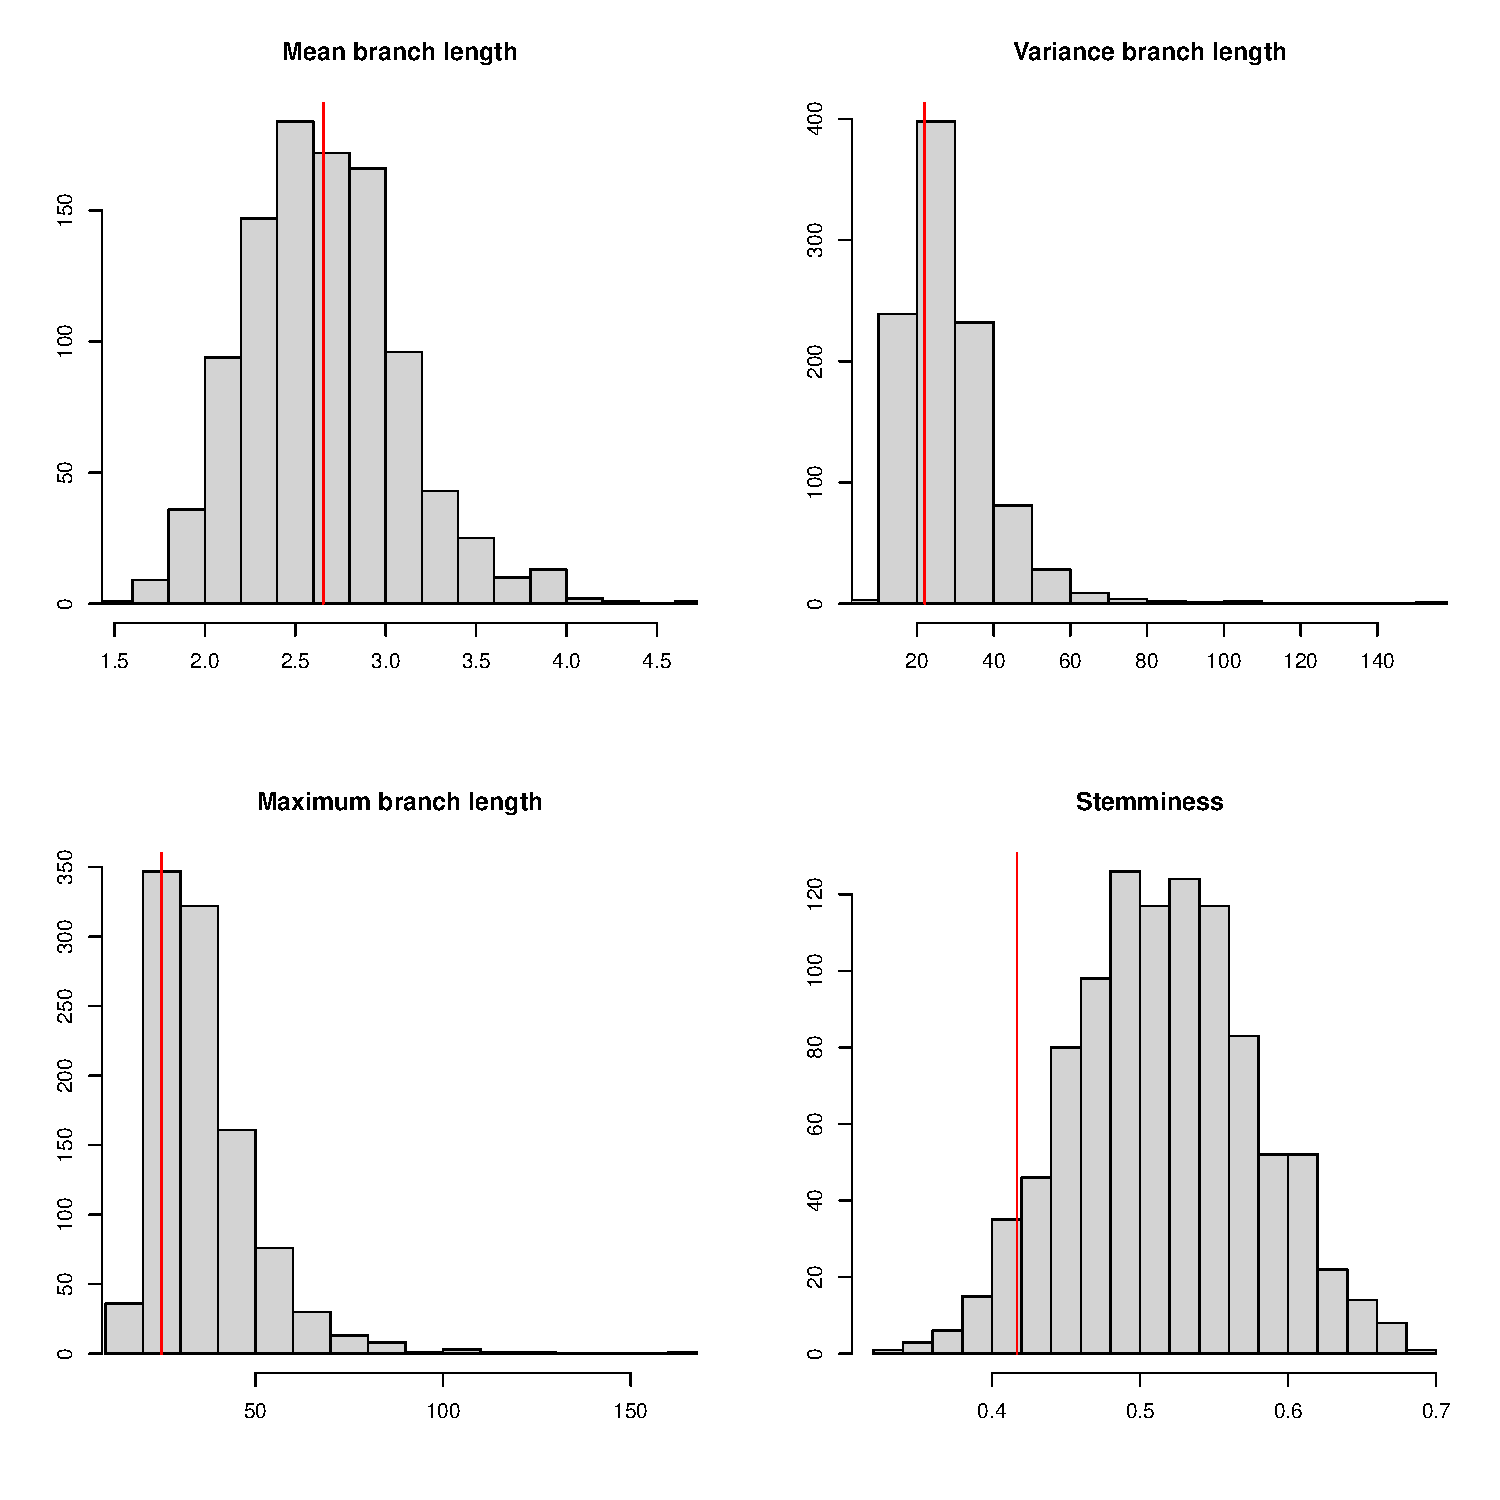
\includegraphics[width=10cm]{examplePPCheck2.pdf}
\end{center}
\caption{Example of posterior predictive analysis.
(A) Inference using incorrect model. 
(B) Inference using correct model.
\label{fig:ppCheck}}
\end{figure}


Posterior predictive assessment is a popular way to perform
model diagnostics in Bayesian statistics \citep{Meng1994,Gelman1996}.
It is frequently used for example in infectious disease epidemiology modeling \citep{Didelot2017b,Whittles2017,gibsonComparisonAssessmentEpidemic2018}.
We therefore sought to apply it to the phylogenetic dating problem, using 
four carefully chosen summary statistics (see Methods): the mean of branch lengths,
variance of branch lengths, maximum of branch lengths and the tree stemminess.
The latter is defined as the sum of lengths of 
internal branches divided by the total sum of branch lengths, with high values usually indicating
variations in population size \citep{fialaFactorsDeterminingAccuracy1985,Didelot2009d}.

A dated phylogeny was simulated including 100 leaves uniformly distributed between 2010 and 2020, 
under the heterochronous coalescent model \citep{Drummond2002}
with constant population size $N_\mathrm{e}g=1$ year (Figure \ref{fig:exampleResid}A). 
We applied the additive relaxed clock model \citep{Didelot2021} to this dated phylogeny,
with mean clock rate $\mu=10$ substitutions per year and relaxation parameter $\omega=5$ (Equation \ref{eq:arc}).
Consequently, some branches had many more or less substitutions compared to what would be expected
under a strict clock model with $\mu=10$, and the probabilities of these branches
under this model would be low (Figure \ref{fig:exampleResid}B). Nevertheless, a root-to-tip regression seemed
very satisfactory, with $R^2=0.94$ and $p<10^{-4}$ for 
a date randomization test (Figure \ref{fig:exampleS1}).

We applied BactDating \citep{Didelot2018} to reconstruct the dated tree twice: first 
incorrectly using a strict clock model (Equation \ref{eq:sc}) and second
correctly using the additive relaxed clock model (Equation \ref{eq:arc}).
In the first case, the clock rate was estimated to be $\mu=10.5$ [9.4;11.6] and the root date 
2008.6 [2008.1;2009.1].
In the second case, the clock rate estimated to be $\mu=11.3$ [8.8;14.1], 
the root date was 2008.9 [2007.7;2009.8]
and the relaxation parameter was $\omega=6.4$ [4.2;8.9]. 
In both cases the values are approximately correct. 
BactDating includes a procedure to perform model comparison by computing
the deviance information criterion (DIC) of each model \citep{Spiegelhalter2002}.
Here the strict clock model had a DIC of 1072.41, whereas the relaxed clock model
had a DIC of 759.86, indicating strong support for the latter. 
This model comparison approach works well here 
since the data was generated here using the relaxed clock model.
However, model comparison is not useful 
more generally to diagnose a single fit without comparison.

The posterior predictive check for the incorrect model diagnosed an issue on
two summary statistics: the variance of the branch lengths and the tree 
stemminess (Figure \ref{fig:ppCheck}A). On the other hand, when the correct model was
used, the posterior predictive assessment did not detect any issue for any of the four
summary statistics (Figure \ref{fig:ppCheck}B). 
The posterior predictive assessment can also be applied more or less directly in the 
case where inference was performed using for example maximum likelihood methods,
either by replacing the posterior samples with the point estimate or by building a
pseudo-posterior (see Methods and next section). 

\subsection*{Residual analysis}

Another diagnostic approach is to consider the distribution of residuals after fitting a model.
This methodology is especially reminiscent of regression models
\citep{coxGeneralDefinitionResiduals1968,dunnRandomizedQuantileResiduals1996},
but has also previously been applied more generally for example to
epidemic models \citep{lauNewModelDiagnostics2014} or 
Hidden Markov Models \citep{zucchini2009hidden,buckbyModelCheckingHidden2020}.
Here we apply this approach to the problem of dating a phylogeny (see Methods), starting first with the case
where the dating was estimated using Bayesian inference and then extending to the case of 
dating using optimization inference. 

\begin{figure}[p!]
\begin{center}
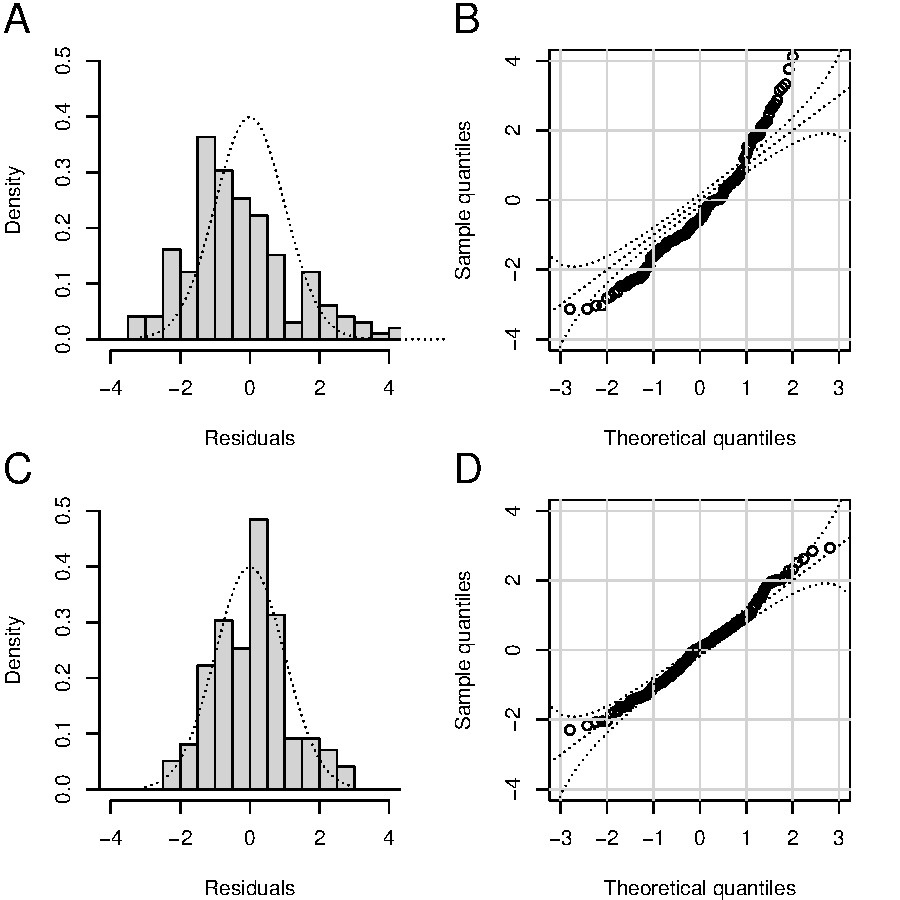
\includegraphics[width=10cm]{exampleResid.pdf}
\end{center}
\caption{Example of residual analysis for a Bayesian inferred dated phylogeny.
(A) Distribution of residuals after inference under a strict clock model. 
(B) QQ plot of residuals after inference under a strict clock model.
(C) Distribution of residuals after inference under a relaxed clock model. 
(D) QQ plot of residuals after inference under a relaxed clock model.
\label{fig:exampleResid}}
\end{figure}

We consider the same two fits as in the previous section, one from the incorrect strict clock model
and one from the correct relaxed clock model. 
When looking at a single sample from the posterior using the incorrect model,
the residuals for the branches were not distributed as Normal(0,1) (Figure \ref{fig:exampleResid}A)
and a QQ plot revealed significant deviation (Figure \ref{fig:exampleResid}B). 
The Anderson-Darling test rejects the hypothesis of standard normality of the residuals ($p<10^{-5}$).
The same residual analysis performed on multiple samples from the posterior showed that they all
had p-values below 0.05, with a median p-value $p<10^{-5}$ (Figure \ref{fig:exampleS2}A).
%We repeated the same analysis incorrectly assuming a strict clock model using 
%LSD \citep{To2016}, node.dating \citep{Jones2017}, treedater \citep{Volz2017} and TreeTime \citep{Sagulenko2018},
%all of which led to similar results (Figure \ref{fig:exampleS2}). 
The residuals for a single sample from the posterior using the correct model
looked approximately distributed as they should be both when plotting them against
their theoretical distribution (Figure \ref{fig:exampleResid}C) and when constructing a QQ plot (Figure \ref{fig:exampleResid}D).
The Anderson-Darling test did not reject the hypothesis of standard normality of the residuals ($p=0.465$).
Repeating this residual analysis on multiple samples from the posterior showed that only 5.1\% of 
them had p-values below 0.05, and the median p-value was $p=0.513$ (Figure \ref{fig:exampleS2}B).

\begin{figure}[p!]
\begin{center}
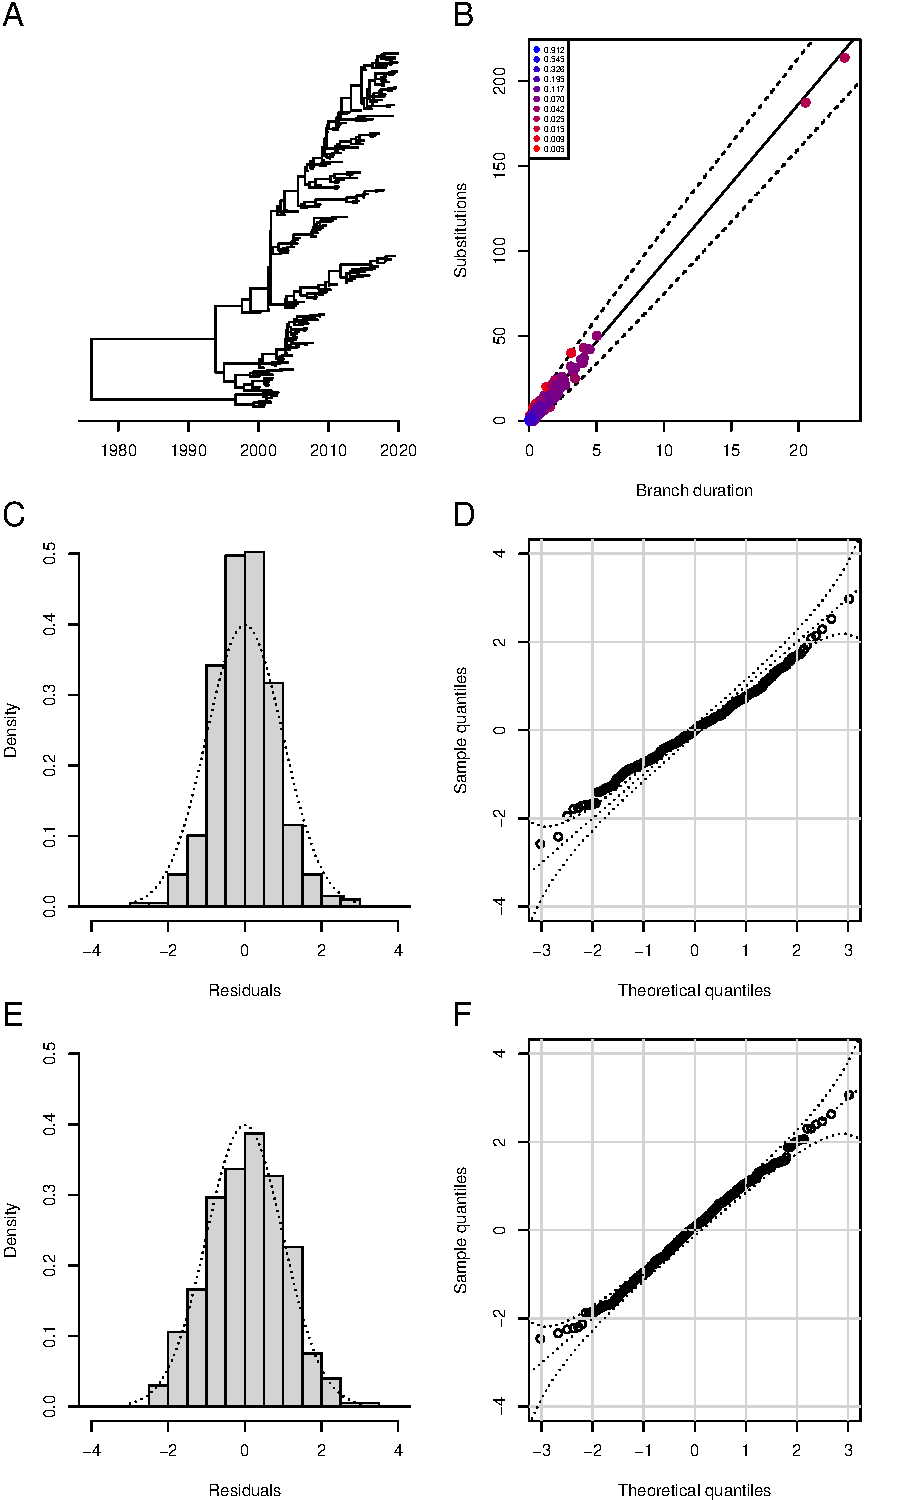
\includegraphics[width=10cm]{exampleML.pdf}
\end{center}
\caption{Example of residual analysis for a maximum-likelihood (ML) dated phylogeny.
(A) Simulated dated phylogeny. (B) Likelihood of substitutions in the ML tree.
dated phylogeny. 
(C) Distribution of residuals in the ML tree. 
(D) QQ plot of residuals in the ML tree.
(E) Distribution of residuals in a tree from the pseudo-posterior. 
(F) QQ plot of residuals in a tree from the pseudo-posterior.
\label{fig:exampleML}}
\end{figure}

We want to apply a similar residual analysis as before in the case of a point-estimated dated tree,
for example using maximum-likelihood (ML) techniques. To illustrate this, we consider the dated
tree in Figure \ref{fig:exampleML}A and apply to it substitutions according to a strict clock model
(Equation \ref{eq:sc}) with rate $\mu=10$ per year. The dated tree was inferred from this substitution data
using treedater \citep{Volz2017} under the correct model, including estimation of the clock rate at 
$\mu=9.32$ and of the root date at 1972.83, which were close to the correct values.
The likelihood of each branch is shown in Figure \ref{fig:exampleML}B.
We computed the residuals for this ML tree as before and compared them the their expected
Normal distribution, see Figures \ref{fig:exampleML}C and \ref{fig:exampleML}D.
It is visually clear that the residuals are underdispersed, and indeed the Anderson-Darling test 
had a p-value of $4\cdot10^{-4}$. This underdispersion of residuals is expected when performing 
ML inference as can be seen if we consider a simpler independently and identically 
distributed model instead of a tree model (see Methods). This complicates the analysis of residuals
compared the the previous Bayesian case, since we no longer have a straightforward expected 
distribution for the residuals. 
%
To remedy this problem, and bridge the gap between Bayesian and 
ML inference, we propose to generate an approximate Bayesian posterior sample centered
around the ML inference (see Methods). The residuals for a single sample from this pseudo-posterior
are shown in Figures \ref{fig:exampleML}E and \ref{fig:exampleML}F, from which it can be seen
that they follow the expected Normal distribution. Indeed the Anderson-Darling test had a p-value
of 0.42. As previously, we can compute such a p-value for all samples in the pseudo-posterior,
which resulted in a posterior distribution of p-values (Figure \ref{fig:exampleMLSup}) with 2.7\% of 
values below 0.05, and the median p-value was $p=0.57$.

\subsection*{Benchmarking}

% latex table generated in R 4.5.1 by xtable 1.8-4 package
% Mon Jul  7 11:43:16 2025
\begin{table}[ht]
\centering
\begin{tabular}{|r|r|r|r|r|r|}
   \hline
Method & Test & Given nothing & Given root & Given rate & Given root and rate \\ 
   \hline
BactDating & PPcheck & 0 & 1 & 1 & 1 \\ 
   & Residuals & 0 & 1 & 0 & 1 \\ 
  treedater & PPcheck & 0 & 1 & 0 & 1 \\ 
   & Residuals & 4 & 5 & 2 & 5 \\ 
  node.dating & PPcheck & 23 & 3 & 28 & 2 \\ 
   & Residuals & 20 & 0 & 24 & 0 \\ 
  TreeTime & PPcheck & 23 & 1 & 35 & 2 \\ 
   & Residuals & 35 & 3 & 40 & 2 \\ 
  LSD & PPcheck & 0 & 1 & 0 & 1 \\ 
   & Residuals & 4 & 2 & 4 & 3 \\ 
   \hline
\end{tabular}
\caption{Number of false positives found amongst a set of 100 replicates. Five different methods were used (BactDating, treedater, node.dating, TreeTime and LSD)
and two different tests (posterior predictive check and residual analysis). Each method was applied in four different conditions: given the correct root, given the
correct rate, given both or given neither.} 
\label{tab:falsePos}
\end{table}


We simulated 100 datasets, each with 100 leaves 
uniformly distributed between 2010 and 2020, 
constant population size $N_\mathrm{e}g=1$ year and 
a strict clock model with  clock rate $\mu=10$ substitutions per year.
For each dataset, we performed dating using five methods: 
BactDating \citep{Didelot2018}, treedater \citep{Volz2017},
node.dating \citep{Jones2017}, TreeTime \citep{Sagulenko2018} and LSD \citep{To2016}.
In each case the dating was performed under four conditions:
with the root given, with the rate given, with both given and with neither given.
Finally, for each inference we computed the p-value according to the posterior
predictive analysis and residual analysis as described previously. We counted the number
of times that the p-values were below 5\% and the results are shown in 
Table \ref{tab:falsePos}. The number of problems diagnosed was low in all situations
for BactDating,treedater and LSD, which is as expected since the same model was used
for simulation and inference. 
On the other hand, both node.dating and TreeTime
produced results for which issues were diagnosed using
both the posterior predictive check and the residual analysis. However, these
issues were detected only when the root was not provided, suggesting that they
were caused by a misidentification of the correct root. 

\subsection*{Confounding effect of population structure} 

TODO: simulate confounding situation, apply diagnosis

\subsection*{Real data examples}

TODO: find two or three examples of dated tree to diagnose

\section*{DISCUSSION}

TODO 

%\begin{figure}[p!]
%\begin{center}
%A\hspace*{6cm}B\hspace*{6cm}~\\
%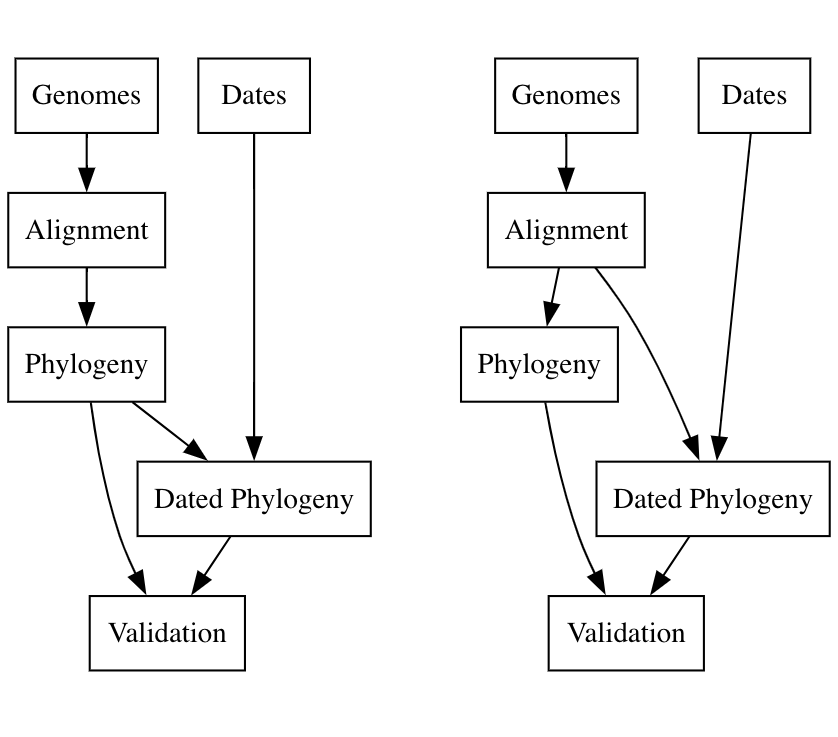
\includegraphics[width=10cm]{fig1.png}
%\end{center}
%\caption{(A) General approach for diagnostics of a dated phylogeny built by dating the nodes of a standard phylogeny. (B) General approach for diagnostics of a dated phylogeny built directly from a sequence alignment.
%\label{fig:approach}}
%\end{figure}
%
%We want to diagnose a dated phylogeny $\mathcal{D}$, previously constructed using
%any method. We propose to do so by comparing the dated phylogeny $\mathcal{D}$ with 
%an undated phylogeny $\mathcal{L}$. 
%If the method used to construct $\mathcal{D}$ involved dating the nodes of an undated
%phylogeny, for example TreeTime \citep{Sagulenko2018} or treedater \citep{Volz2017}, 
%then this is readily available for diagnostics and we therefore focus on this case in this article
%(Figure \ref{fig:approach}A). However, the diagnostics methodology
%above can also be applied to methods that build a dated phylogeny directly from the alignment
%such as BEAST \citep{Suchard2018},
%simply by constructing a separate undated phylogeny from the same alignment using
%for example PhyML \citep{Guindon2010} or RAxML \citep{Stamatakis2015} 
%(Figure \ref{fig:approach}B). 
%But not clear what to do if the dated phylogeny and undated phylogeny don't have the same topology. Maybe what would be better would be to do ancestral state reconstruction given the dated tree, so that substitutions can be counted on the tree and eg residuals calculated. Could be done using eg FastML.
%For each branch in the dated phylogeny $\mathcal{D}$ we can
%consider its inferred length, the number of substitutions happening on that branch in the standard phylogeny
%$\mathcal{L}$, and the model and parameters used when building the dated phylogeny $\mathcal{D}$,
%in order to compute a residual for that branch (see Methods). If the inference is valid,
%these residuals will follow their theoretical distribution
%\citep{coxGeneralDefinitionResiduals1968,dunnRandomizedQuantileResiduals1996}. 
%We use this property as a way to test the validity of the dated phylogeny $\mathcal{D}$.

\section*{MATERIALS AND METHODS}

\subsection*{Molecular clock models}

The molecular clock model determines the distribution of number of substitutions $l_i$ on a branch of the dated
tree with duration $d_i$. We consider four types of molecular clock models, for each combination of whether
the values $l_i$ are discrete or continuous and whether the clock model is strict or relaxed. 
In the discrete strict clock
model \citep{Zuckerkandl1962} with rate $\mu$,
substitutions occur on the branches as a Poisson process with rate $\mu$ and therefore:

\begin{equation}
l_i \sim \mathrm{Poisson}(d_i \mu)
\label{eq:sc}
\end{equation}

A continuous version of the strict clock model can be formed based on a Gamma process with the same mean and variance \citep{Didelot2021}:

\begin{equation}
l_i \sim \mathrm{Gamma}(d_i \mu,1)
\label{eq:csc}
\end{equation}

Strict clock models are based on the assumptions that the substitution rate is constant throughout the branches
of the tree, but this is not always true in which case a relaxed clock model can be used which allows
the rate to vary \citep{Drummond2006}. In particular here we use the additive relaxed clock model \citep{Didelot2021},
in which $\mu$ is the mean clock rate and $\omega$ determines how much this rate varies on the branches.
The discrete version of this model is given by: 

\begin{equation}
l_i \sim \mathrm{NegativeBinomial}\left(\frac{d_i \mu}{\omega},\frac{1}{1+\omega}\right)
\label{eq:arc}
\end{equation}

A continuous additive relaxed clock model can again be defined by considering a Gamma process with the same mean and variance:
\begin{equation}
l_i \sim \mathrm{Gamma}\left(\frac{d_i \mu}{1+\omega},1+\omega\right)
\label{eq:carc}
\end{equation}

Note that throughout this article Gamma distributions are parametrized by shape and scale and Negative Binomials 
by number of successes and probability of success. In the four models we have that the mean of $l_i$ is equal to
$d_i \mu$. The variance of $l_i$ is equal to its mean in the two strict clock models, and equal to its mean 
times $(1+\omega)$ in the two relaxed clock models.

\subsection*{Posterior predictive checks}

When applied to the phylogenetic dating problem, posterior predictive checking requires
to simulate many undated phylogenies from the posterior sample of dated phylogeny,
and comparing them to the observed undated phylogeny from which inference was performed.
Simulation is done using the same clock model as was used for inference (Equations \ref{eq:sc} to \ref{eq:carc})
and using the posterior inferred parameters. Posterior predictive assessment can also be performed
following inference from a maximization method, using the single inferred dated tree and parameters as 
starting point for all simulations. 
The comparison of simulated and observed phylogenies is done on the basis of summary statistics, and
here we used the following four: mean of branch lengths, variance of branch lengths,
maximum of branch lengths and stemminess \citep{fialaFactorsDeterminingAccuracy1985}. 
These summary statistics were selected to represent different aspects of the phylogeny without
being too numerous to avoid worsening the multiple testing issue, and we found them to be a useful
choice in practice but we do not claim that they are in any way optimal.
For each summary statistics, an empirical p-value is computed representing how extreme the 
observed phylogeny is compared to the set of simulated ones. 
These p-values can then be combined into a single p-value while controlling for multiple testing.
We used a false discovery rate (FDR) correction \citep{Benjamini1995} although other options would also be 
possible for example using a harmonic mean p-value \citep{wilsonHarmonicMeanPvalue2019}.

\subsection*{Computation and analysis of residuals}

We want to diagnose a dated phylogeny $\mathcal{D}$ by comparison with an undated phylogeny $\mathcal{L}$. We start by considering the case where the dated phylogeny $\mathcal{D}$ is a single sample from the posterior distribution $p(.|\mathcal{L})$ obtained for example using BactDating \citep{Didelot2018}.
Let $d_i$ be the duration of a given branch in $\mathcal{D}$ and $l_i$ be the number of substitutions on the corresponding branch of $\mathcal{L}$, that is the branch that separates the leaves in the same way. There is a unique corresponding branch in $\mathcal{L}$ for all branches in $\mathcal{D}$ except for the two branches $a$ and $b$ connected to the root of $\mathcal{D}$ for which there is only a single corresponding branch $x$. We therefore split the substitutions on $x$ proportionally between the two branches $a$ and $b$ by defining:

\begin{equation}
l_a = \frac{l_x d_a}{d_a+d_b}\mathrm{~and~}l_b = \frac{l_x d_b}{d_a+d_b}
\end{equation}

The distribution of $l_i$ given $d_i$ is given by the molecular clock model. 
Let us for now consider that the distribution
is continuous (as in Equations \ref{eq:csc} and \ref{eq:carc}) and we will return later to the discrete case 
(as in Equations \ref{eq:sc} and \ref{eq:arc}). 
Instead of a specific model, we consider the general case where
$F_i(l_i)$ is the cumulative distribution function of $l_i$ given $d_i$.
Let $u_i$ denote the uniform residual for the observation $l_i$, defined as:

\begin{equation}
u_i=F_i(l_i)=p(L_i\leq l_i|d_i)
\label{eq:unif-resid}
\end{equation}

If the inference is valid, then the uniform residual $u_i$ 
should be distributed as Uniform(0,1), because for any random variable $X$ with cumulative distribution function $F$ we have that $U=F(X)$ is Uniform(0,1). 
However, it is difficult to assess how close to zero or one a value needs to be in order to be 
an outlier. 
We therefore define the normal residuals $n_i$, analogous to the residuals commonly used in 
regression models \citep{coxGeneralDefinitionResiduals1968,dunnRandomizedQuantileResiduals1996}. 
The normal residuals are obtained 
by transforming the uniform residuals with the inverse of the cumulative distribution function $\Phi$ 
of a Normal(0,1) random variable:

\begin{equation}
n_i=\Phi^{-1}(u_i)\mathrm{~with~}\Phi(x)=\frac{1}{\sqrt{2\pi}}\int_{-\infty}^x e^{-t^2/2}\mathrm{d}t
\label{eq:norm-resid}
\end{equation}

If the inference is valid, then the normal residuals $n_i$ should be distributed
as Normal(0,1) which is more convenient to work with than the Uniform(0,1) for uniform residuals.
The uniform and normal residuals above can be computed directly
when the clock model is continuous (Equations \ref{eq:csc} and \ref{eq:carc}) but when
the clock model is discrete (Equations \ref{eq:sc} and \ref{eq:arc}) we need to make the following
adjustment \citep{dunnRandomizedQuantileResiduals1996,brockwellUniversalResidualsMultivariate2007,lauNewModelDiagnostics2014}:

\begin{equation}
u_i \sim \mathrm{Unif}(F_i(l_i),F_i(l_i+1))
\label{eq:unif-resid-discrete}
\end{equation}

After computation of the uniform residuals $u_i$ and normal residuals $n_i$ for each branch,
we use several methods to assess the validity of the dated phylogeny inference.
The uniform residuals $u_i$ can be plotted as a histogram to compare their
distribution with the theoretical Uniform(0,1) distribution, but as previously noted this can
be difficult to interpret. We therefore prefer to use the normal residuals $n_i$ which can be plotted
as a histogram to compare their distribution with the theoretical Normal(0,1).
A quantile-quantile plot (QQ plot) can be used to compare the distribution of the residuals
to their theoretical distribution.
A p-value can be computed to assess that the normal
residuals are distributed as expected. 
The most commonly used and powerful test of normality 
is the Shapiro-Wilk test \citep{razaliPowerComparisonsShapiroWilk2011},
but it is a composite test for when the mean and variance
are unknown, whereas here we know that the
normal residuals follow the standard normal distribution with
mean 0 and variance 1. We therefore use the
Anderson-Darling simple hypothesis 
test \citep{lewis1961distribution} 
as implemented in the DescTools R package
based on previously published code
\citep{marsagliaEvaluatingAndersonDarlingDistribution2004}. 
%Anderson-Darling simple hypothesis testing was used in \citep{lauNewModelDiagnostics2014} via implementation in package ADGofTest, returns same results as DescTools. Both use the same C code from 
%\citep{marsagliaEvaluatingAndersonDarlingDistribution2004}. 

We have described the diagnosics procedure above as if there was a single posterior
sample $\mathcal{D}$ to diagnose, whereas there would typically be multiple samples
from this posterior available for example from running a Markov Chain Monte-Carlo
method \citep{Didelot2018}. However, the same computation and analysis of residuals
could be performed for each sample as described above. Each statistical test will
return a separate p-value and these can be combined to form a 
a posterior distribution of p-values \citep{streftarisNonexponentialToleranceInfection2012,lauNewModelDiagnostics2014,gibsonComparisonAssessmentEpidemic2018}.
From this posterior distribution of p-values we can compute
various summaries to measure the validity of the inference,
for example the proportion of p-values that are below 0.05
\citep{lauNewModelDiagnostics2014}. Here we prefer instead
to focus on the median of the posterior sample of p-values,
since it can be interpreted more directly as a p-value.

\subsection*{Pseudo-posterior sampling given a point estimate}

We now consider the case where the dated phylogeny $\mathcal{D}$ that we wish
to diagnose was not sampled from the posterior. Instead it may be a point estimate, 
for example the result of maximum likelihood estimation
or a summary tree built from a posterior sample \citep{heledLookingTreesForest2013}
but for which the posterior sample itself is not available.
In this case we propose to first generate approximate 
samples from the posterior before residuals can be computed as described above.
If the residuals were computed directly from the point estimate, they would not follow the same distribution as in Equations
\ref{eq:unif-resid} and \ref{eq:unif-resid-discrete}.
To explain and illustrate this, let us first consider the discrete strict clock model (Equation \ref{eq:sc})
with known mutation rate $\mu=1$
and that the true branch durations $d_i$ are independent and identically
distribution as:
\begin{equation}
d_i \sim \mathrm{Gamma}(k=2,\theta=2)
\end{equation}
Let $\hat{d_i}$ be a branch length in $\mathcal{D}$, on which there are $l_i$ substitutions in the undated phylogeny $\mathcal{L}$. 
The true residuals of each branch are distributed as expected (Figure \ref{fig:iid}A)
and so are the residuals based on a posterior sample of $d_i$ given $l_i$ (Figure \ref{fig:iid}B).
If $\hat{d_i}$ is a maximum likelihood estimate of $d_i$ then
$\hat{d_i}=l_i/\mu$.
The residuals of the data points $l_i$ against the estimates $\hat{d_i}$ are
underdispersed, because the maximum likelihood estimates are overfitted (Figure \ref{fig:iid}C).
It is however possible in this case to recover the exact correct residuals by sampling from
the posterior. 
By conjugacy of the Gamma prior and Poisson likelihood, we can deduce that the posterior of $d_i$ is:
\begin{equation}
d_i \sim \mathrm{Gamma}\left(k+\hat{d_i} \mu,\frac{\theta}{1+\theta \mu}\right)
\end{equation}
We can simulate from this distribution to get a posterior sample $d_i$, from which we can then compute the residuals as 
described previously which will be distributed as in 
Equations \ref{eq:unif-resid} and \ref{eq:unif-resid-discrete} (Figure \ref{fig:iid}D).

The case described above works exactly but is idealised for two reasons.
Firstly the branch durations $d_i$ are neither independent nor identically distributed,
but rather related through each other via the coalescent process. Secondly
the clock is not usually strict with a known rate so that
a posterior would not be analytically available. 
However, we can follow
a similar idea of generating a pseudo-posterior sample centered on the given
point estimate $\mathcal{D}$. To do so, we perform a short run of BactDating \citep{Didelot2018}
for the input phylogeny $\mathcal{R}$ 
with branch lengths equal to
the lengths in $\mathcal{D}$ multiplied by the clock rate 
$\hat \mu$ estimated when the dated tree was inferred. 
If this estimate is not available, a simple maximum likelihood
estimator can be used instead: 
\begin{equation}
\hat \mu = \frac{\sum_i l_i}{\sum_i d_i}
\end{equation}
Since the branch lengths in $\mathcal{R}$ are continuous, 
inference is performed under the 
continuous version of the strict clock model (Equation \ref{eq:csc}).  
The clock rate is fixed equal to its previous estimate $\hat \mu$, and the coalescent rate $\alpha$
is fixed equal to either its previous estimate (if available) or
the maximum likelihood estimator:
\begin{equation}
\hat \alpha = \frac{\sum_{i=2}^{2n-1}k_i (k_i-1)(t_i-t_{i+1})}{2(n-1)}
\end{equation}
Note that this corresponds to the mean of the posterior distribution of $\alpha$ 
assuming an improper $\mathrm{InvGamma}(0,\infty)$ prior on $\alpha$ so that posterior is:
\begin{equation}
\alpha \sim \mathrm{InvGamma}\left(n-1, \frac{2}{\sum_{i=2}^{2n-1}k_i (k_i-1)(t_i-t_{i+1})}\right)
\end{equation}
The posterior sample returned by BactDating can be thought of as a pseudo-posterior centered
on the point estimate $\mathcal{D}$, from which residuals can be computed as in the Bayesian case.
An alternative would be to use a 
parametric bootstrap \citep{efronBayesianInferenceParametric2012}. Generating a thousand bootstrapped
datasets is easy simply by application of one of the molecular clock models (Equations
\ref{eq:sc} to \ref{eq:carc}) to the point estimate $\mathcal{D}$, but inference would then have
to be performed for each bootstrapped dataset which is not computationally
attractive for the size of datasets considered here. 

\subsection*{Data simulation}

The unstructured datasets were simulated by first sampling from the 
heterochronous coalescent model \citep{Drummond2002} and then applying one of the molecular
clock models (Equations \ref{eq:sc} to \ref{eq:carc}). 
We tested several approaches to the simulation of confounding structured datasets \citep{Murray2016}, 
including using 
DetectImports \citep{Didelot2022detectimports} and using Master \citep{Vaughan2013} to 
simulate under the structured coalescent model \citep{Nordborg1997}, but these methods would
typically not cause enough confounding effect for our purposes. We therefore implemented our own
simulation method using mlesky \citep{Didelot2023mlesky} to simulate each population component genealogy $\mathcal{G}$
under a coalescent model with a non-constant population size $N(t)$, so that its probability follows:
\begin{equation}
p(\mathcal{G}|N(t))=\exp \left(-\int_{-\infty}^{\infty}\mathbbm{1}[A(t)\geq 2]
\frac{A(t)(A(t)-1)}{2N(t)} \mathrm{d}t\right) \prod_{i=1}^{n-1} \frac{1}{N(c_{i})}
\label{eqn:coalescent}
\end{equation}
\noindent where $A(t)$ represents the number of lineages
at time $t$ and $c_i$ represents the times of the nodes.
The size of the $j$-th population component followed 
a previously studied model of clonal expansion \citep{Helekal2021}:
\begin{equation}
N_j(t)=\frac{M_j(t-s_j)^2}{h_j^2+(t-s_j)^2}\mathbbm{1}[t \geq s_j]
\end{equation}
Each population component starts at time $s_j$ with 
size $N(s_j)=0$ and grows logistically up to its maximum $N_j(\infty)=M_j$, with $h_j$ being the time 
taken to reach half of this since $N_j(s_j+h_j)=M_j/2$. 

\subsection*{Real data}

TODO

\subsection*{Implementation}

We implemented the analytical methods described in this paper in a 
new R package entitled \emph{DiagnoDating} which is available
at \url{https://github.com/xavierdidelot/DiagnoDating} for R version 3.5 or later. 
All code and data needed to replicate the results are included in the ``reproducibility'' directory of the \emph{DiagnoDating} repository.

\section*{ACKNOWLEDGEMENTS}

We acknowledge funding from the National Institute for Health Research (NIHR) Health Protection Research Unit in Genomics and Enabling Data.

\newpage
\bibliographystyle{mbe}
\bibliography{/Users/u1775021/all.bib}
%\bibliography{biblio}

\pagenumbering{gobble}
\newpage
%Supplementary Material
\setcounter{figure}{0}
\setcounter{table}{0}
\makeatletter 
\renewcommand{\thefigure}{S\@arabic\c@figure} 
\renewcommand{\thetable}{S\@arabic\c@table} 
\makeatother

\begin{figure}[t!]
\begin{center}
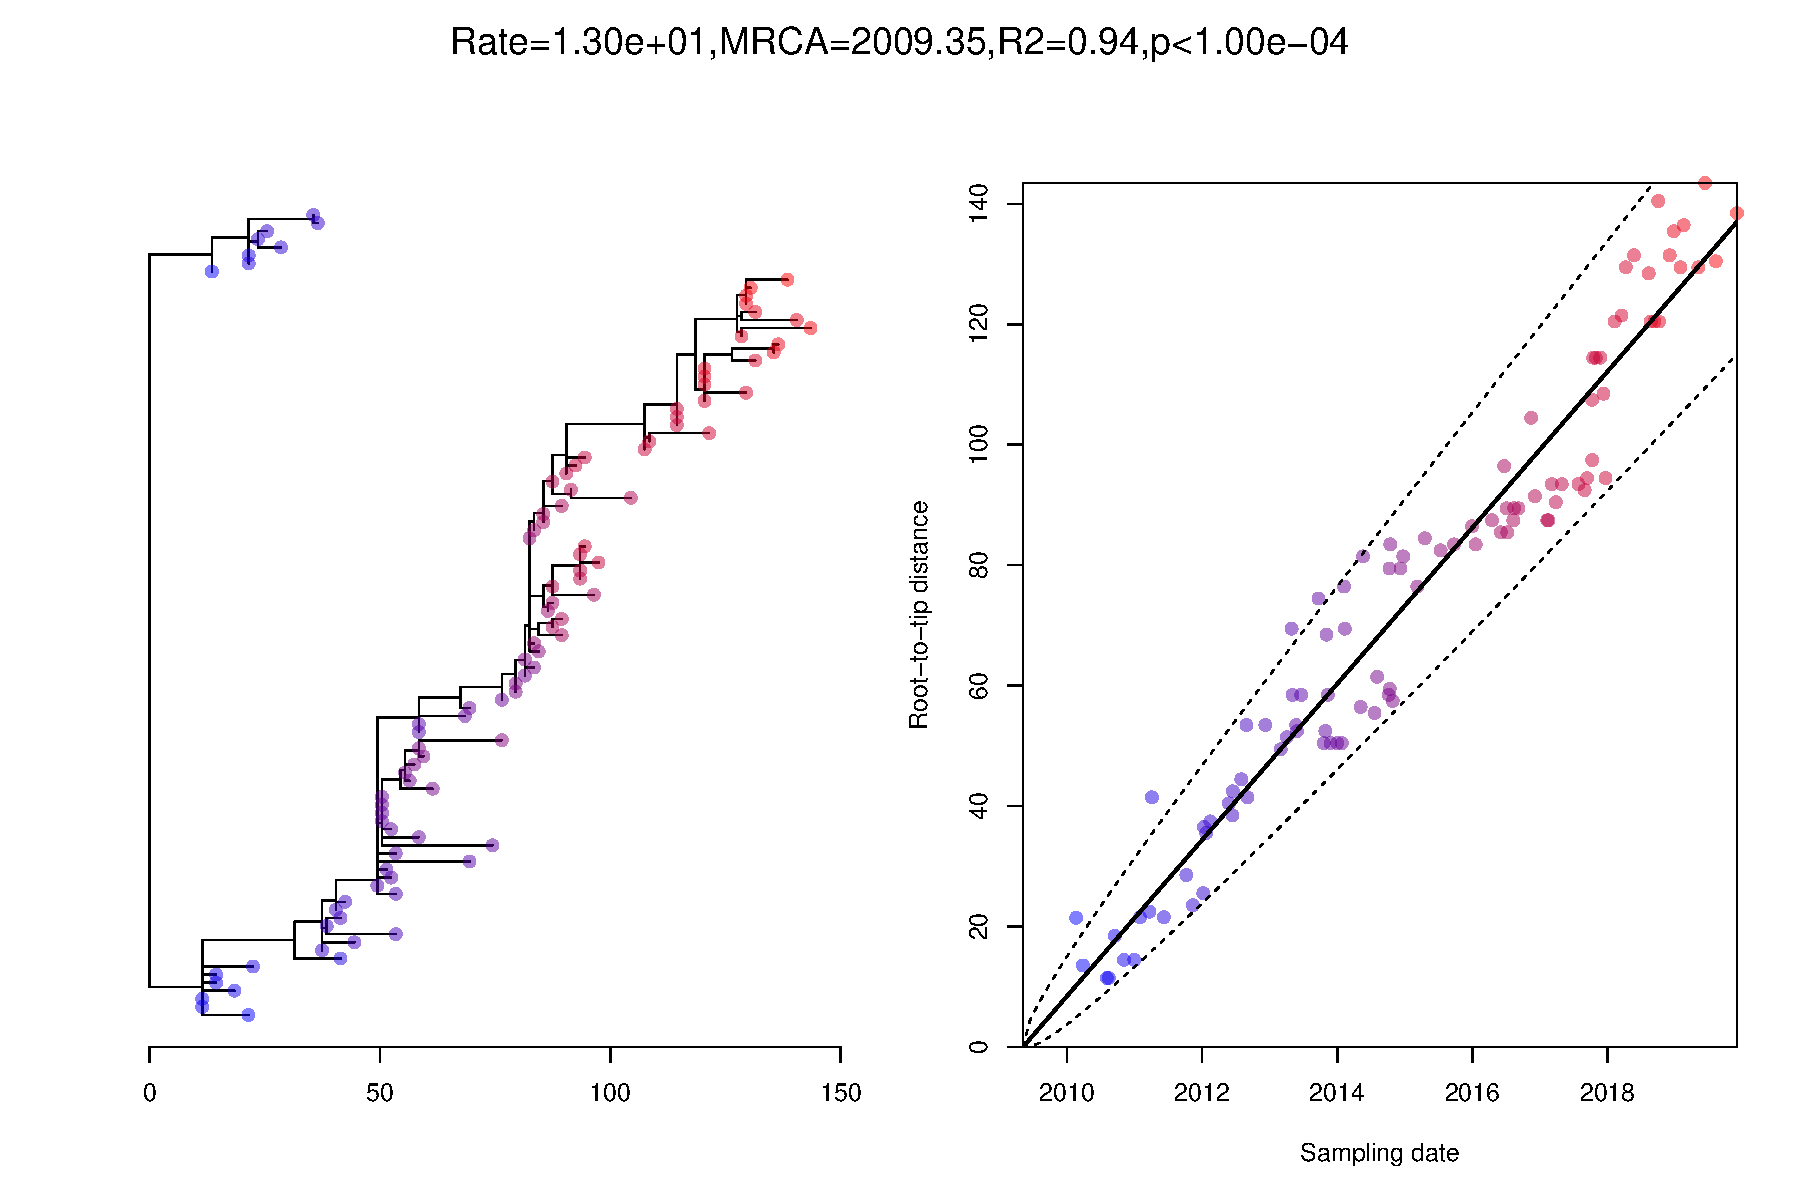
\includegraphics[width=15cm]{exampleS1.pdf}
\end{center}
\caption{Root-to-tip regression analysis for the motivating example.
\label{fig:exampleS1}}
\end{figure}

\begin{figure}[t!]
\begin{center}
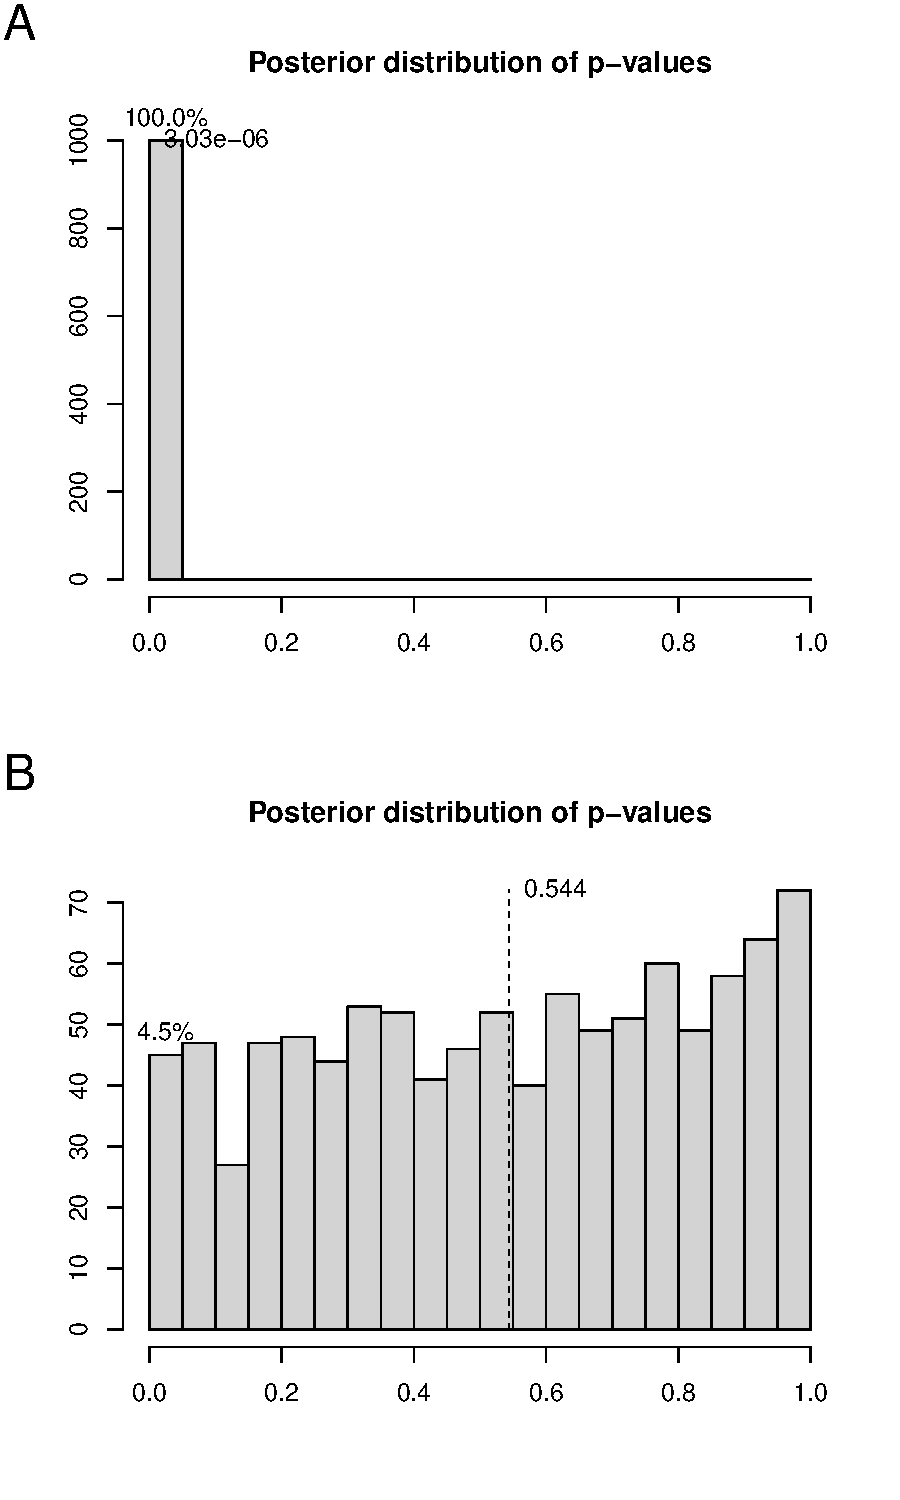
\includegraphics[width=10cm]{exampleS2.pdf}
\end{center}
\caption{Posterior distribution of p-values for inference under the strict clock model (A) and ARC model (B).
%Residuals after application on the motivating example of a strict clock model using LSD (A), node.dater (B), treedater (C) and TreeTime (D).
\label{fig:exampleS2}}
\end{figure}

\begin{figure}[t!]
\begin{center}
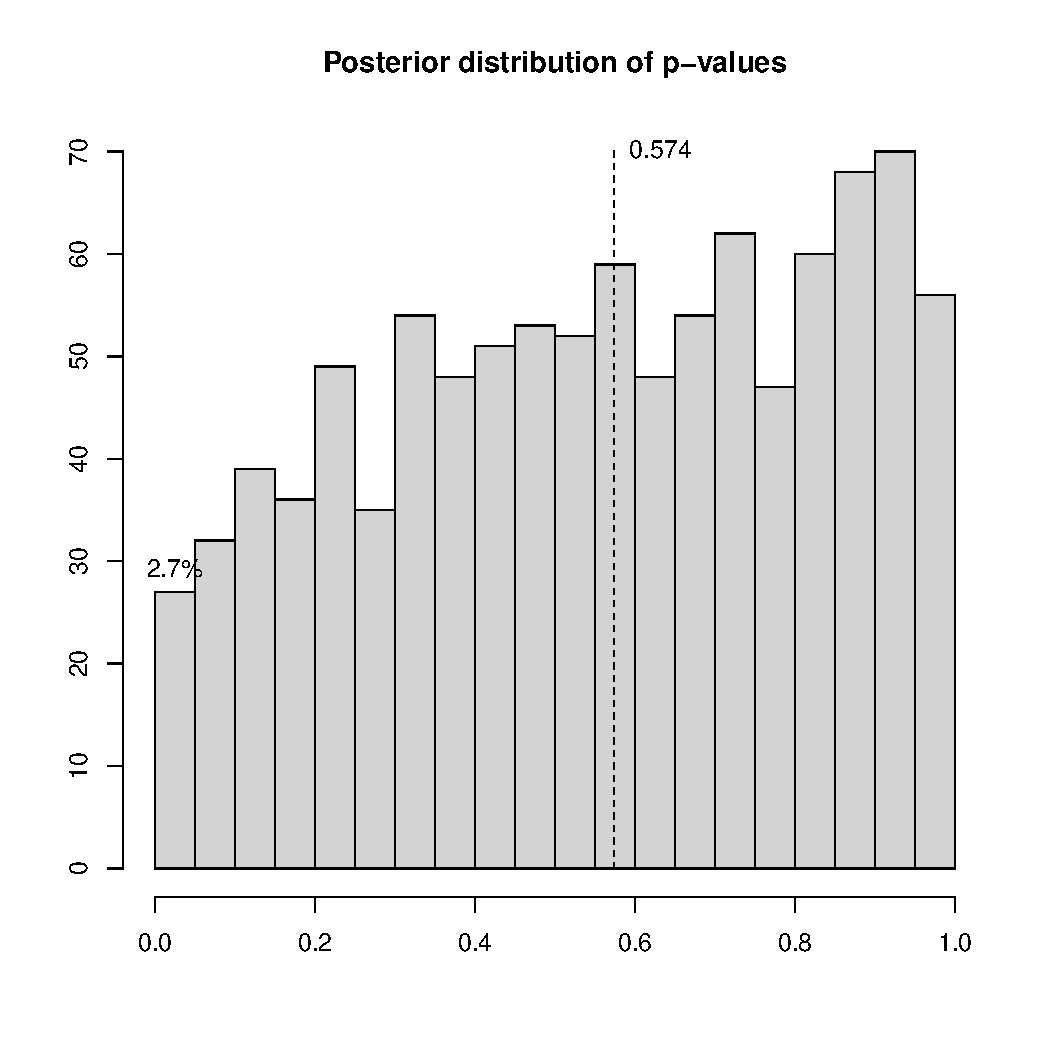
\includegraphics[width=10cm]{exampleMLSup.pdf}
\end{center}
\caption{Posterior distribution of p-values for the pseudo-posterior based on ML inference.
\label{fig:exampleMLSup}}
\end{figure}


\begin{figure}[t!]
\begin{center}
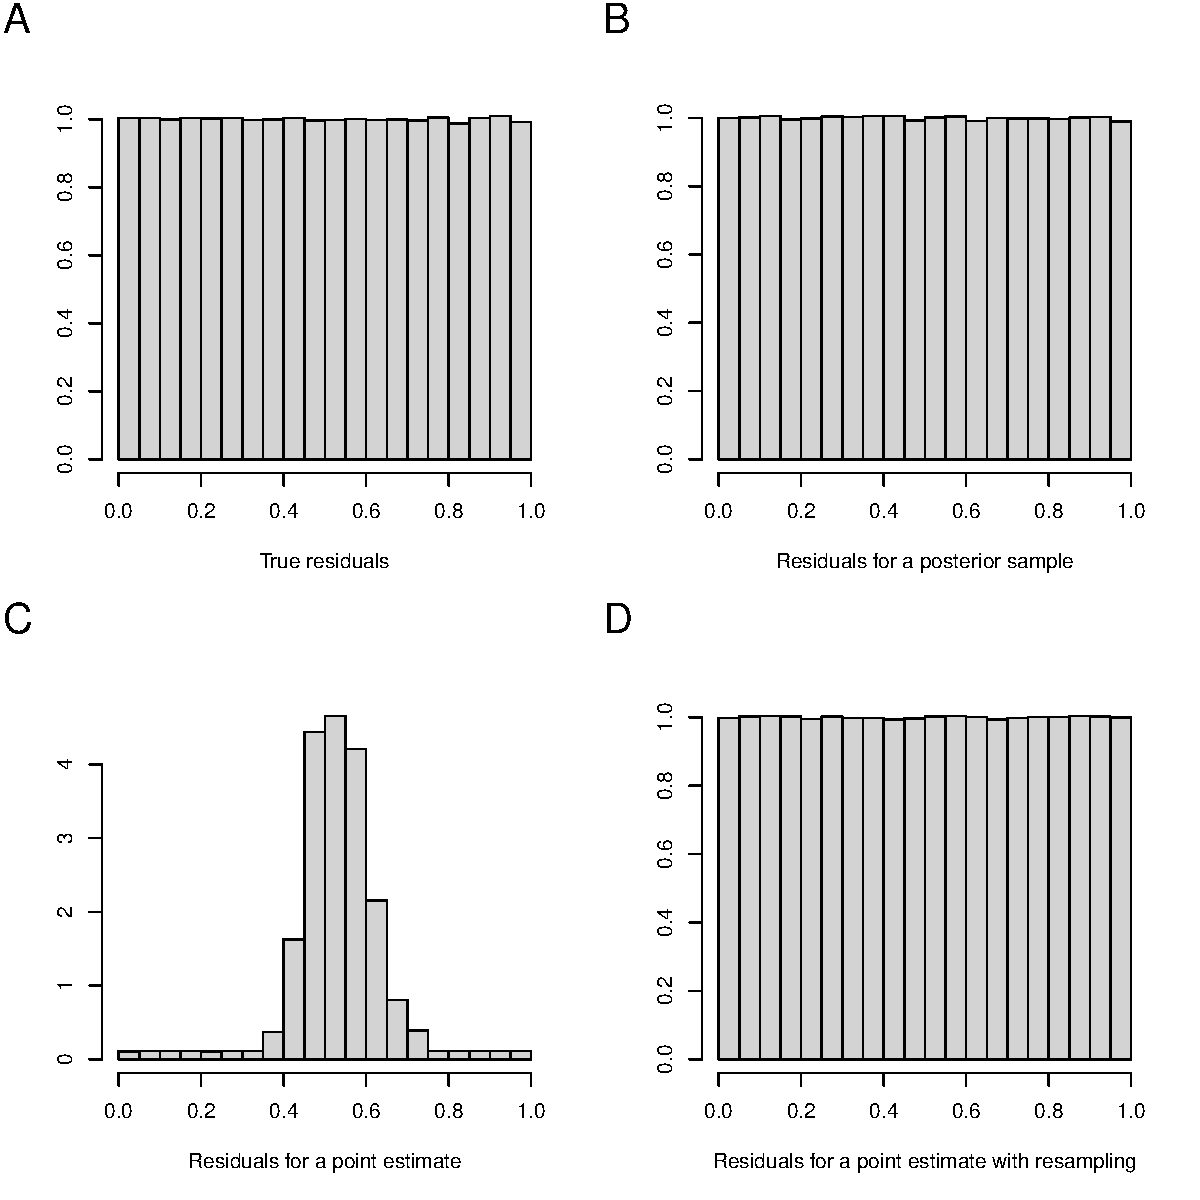
\includegraphics[width=15cm]{iid.pdf}
\end{center}
\caption{Uniform residuals in the independent and identically distributed case. 
(A) True residuals. (B) Residuals based on a posterior sample.
(C) Residuals based on a point estimate.
(D) Residuals based on a point estimate with resampling.
\label{fig:iid}}
\end{figure}


\end{document}

